\documentclass[11pt]{article}
\usepackage[margin=1in]{geometry}
\usepackage{graphicx}
\usepackage{booktabs}
\usepackage{float}
\usepackage{amsmath}
\usepackage[colorlinks=true,urlcolor=blue,citecolor=blue]{hyperref}

\title{Expression of \textit{ESR1} and \textit{ERBB2} Across PAM50 Subtypes in TCGA-BRCA Breast Cancer}
\author{Faris Halilovic}
\date{\today}

\begin{document}
\maketitle

%---------------------------------------------------------------
\section{Introduction}
This report analyzes RNA-seq gene expression data from the TCGA-BRCA project, which contains 1,231 breast cancer and normal breast tissue samples with associated clinical metadata \cite{tcga2012,grossman2016}. The samples include 1,111 primary tumors, 7 metastatic tumors, and 113 solid tissue normals. 

For this project, I choose to focus on two genes with established roles in breast cancer. \textit{ESR1} encodes the estrogen receptor, which promotes growth in tumors positive for hormone receptors and is a target of endocrine therapy. \textit{ERBB2} encodes the HER2 receptor, which is amplified in the HER2-enriched subtype and is a target of anti-HER2 therapies. Because both genes are used to classify breast tumors, their expression is a way to examine the types in this study. My earlier check-in report used \textit{DPM1}, but for this final report I chose \textit{ESR1} and \textit{ERBB2} because their roles in breast cancer are well established and they allow comparison across the PAM50 subtypes. \textit{DPM1} is kept in Table~\ref{tab:summary} for comparison.

%---------------------------------------------------------------
\section{Methods}
RNA-seq counts and sample metadata for TCGA-BRCA were obtained from course-provided files \cite{courseData}. Analyses were performed in R version 4.4.1 using R Markdown. Raw counts were transformed as $\log_2(\text{count}+1)$ for all plots; the summary statistics in Table~\ref{tab:summary} use raw counts. Plots were made with \texttt{ggplot2} (version 4.0.2) \cite{wickham2016} and \texttt{tidyverse} (version 2.0.0). Tables were generated with \texttt{knitr} (version 1.48). The heatmap was created with \texttt{ComplexHeatmap} (version 2.22.0) \cite{gu2016,guBook}, using z-scores of $\log_2$ counts for ten breast cancer marker genes (\textit{ESR1}, \textit{ERBB2}, \textit{GATA3}, \textit{FOXA1}, \textit{PGR}, \textit{MKI67}, \textit{KRT5}, \textit{KRT17}, \textit{CDH1}, and \textit{EGFR}). Samples without a PAM50 label were excluded from the box plot, heatmap, and density plot. Density estimates of \textit{ESR1} expression were calculated for each subtype using the default settings of \texttt{geom\_density}.

%---------------------------------------------------------------
\section{Results}

\subsection{Summary statistics}
Table~\ref{tab:summary} reports summary statistics for \textit{ESR1} and \textit{ERBB2}. The means are well above the median, indicating right-skewed distributions, and \textit{ERBB2} shows a very large maximum (995,067), consistent with high expression in a subset of tumors. \textit{DPM1}, the gene selected from final project check in assignment one had lower and more stable counts than the two breast cancer marker genes.

\begin{table}[H]
\centering
\small
\caption{Summary statistics of raw counts for \textit{DPM1}, \textit{ESR1}, and \textit{ERBB2}.}
\label{tab:summary}
\begin{tabular}{lrrrrr}
\toprule
Gene & Mean & Median & SD & Min & Max \\
\midrule
\textit{DPM1}  & 2416.3 & 2052 & 1459.5 & 312 & 17569 \\
\textit{ESR1}  & 31442.2 & 17561 & 38261.2  & 14  & 270977 \\
\textit{ERBB2} & 46982.5 & 19125 & 105287.5 & 205 & 995067 \\
\bottomrule
\end{tabular}
\end{table}

\subsection{Distribution of \textit{ESR1} expression}
\begin{figure}[H]
\centering
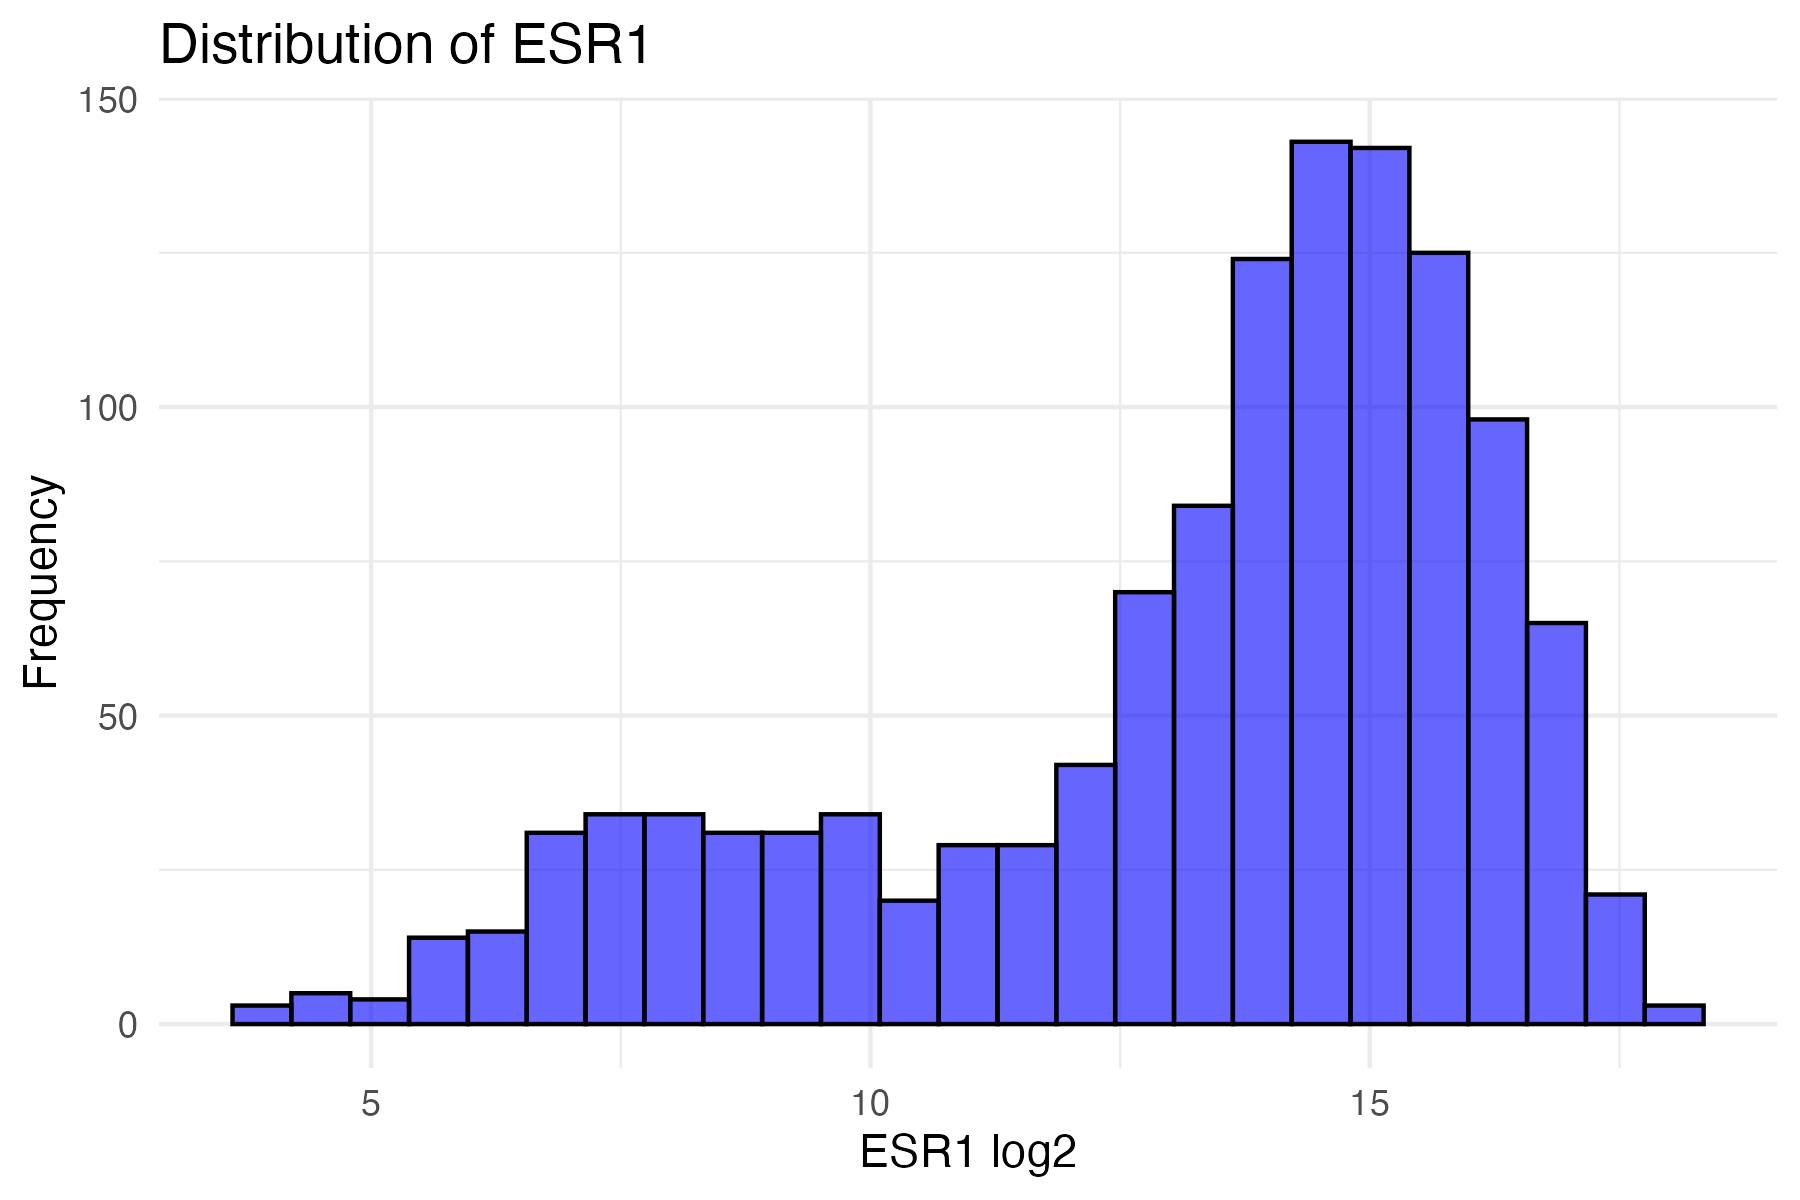
\includegraphics[width=0.75\textwidth]{figures/histogram.png}
\caption{Histogram of \textit{ESR1} expression log2 across all samples.}
\label{fig:hist}
\end{figure}
Expression is bimodal. Most samples formed a large peak at roughly 14--15 $\log_2$ units, while a smaller group clustered at much lower expression around 7--10.

\subsection{Relationship between \textit{ESR1} and \textit{ERBB2}}
\begin{figure}[H]
\centering
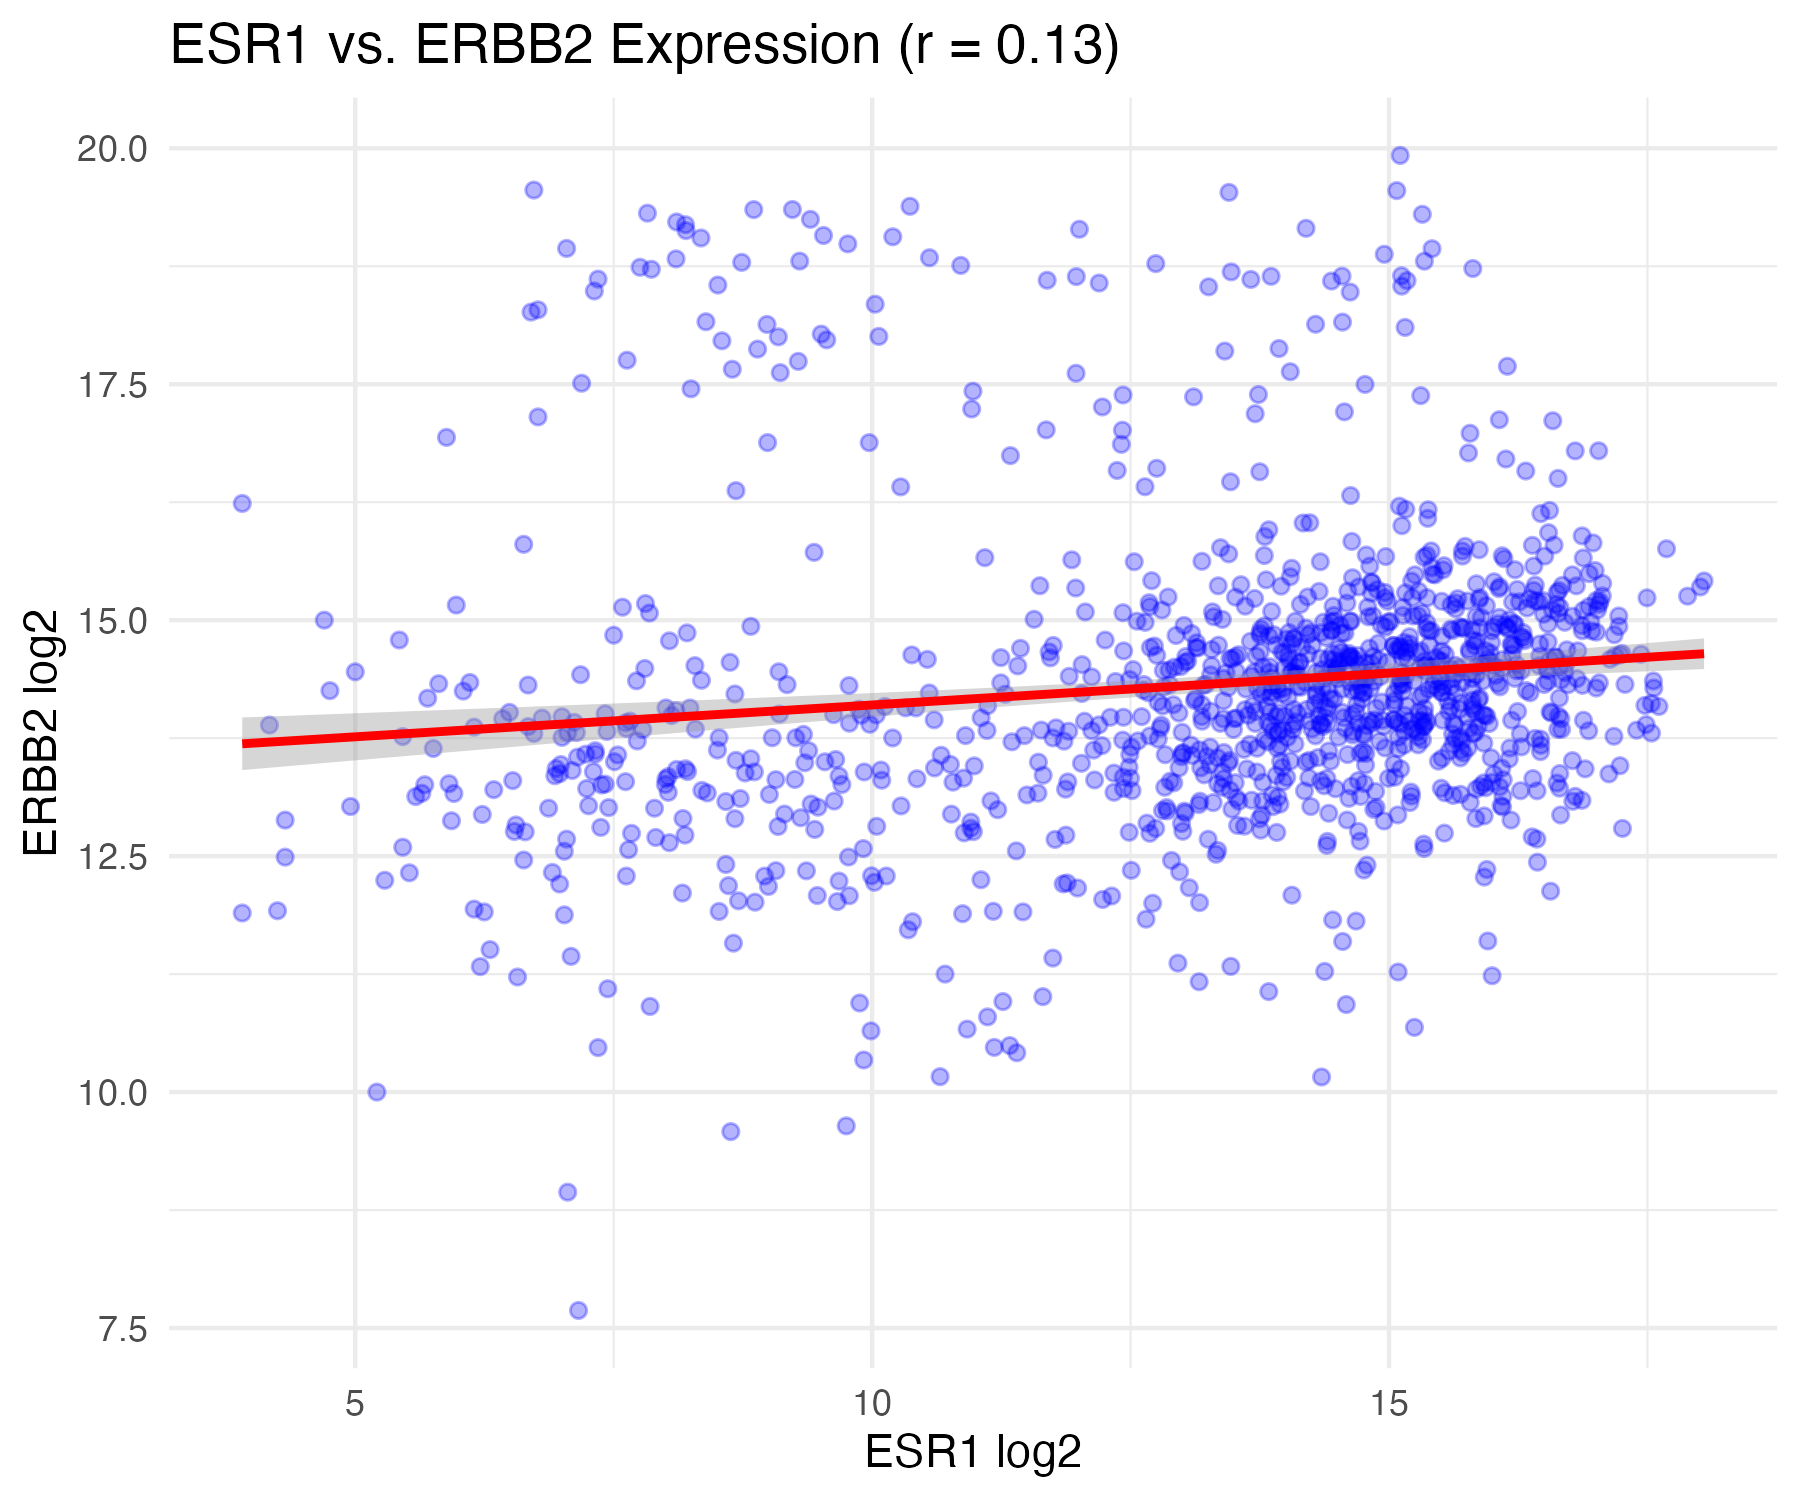
\includegraphics[width=0.75\textwidth]{figures/scatter_plot.png}
\caption{Scatter plot of \textit{ESR1} versus \textit{ERBB2} expression with a linear trend line.}
\label{fig:scatter}
\end{figure}
The two genes showed a weak correlation, therefore \textit{ESR1} expression explains the small variation in \textit{ERBB2}. A group of samples with high \textit{ERBB2} appears across moderate \textit{ESR1} levels, which may represent \textit{ERBB2} amplified tumors.

\subsection{\textit{ESR1} expression by PAM50 subtype}
\begin{figure}[H]
\centering
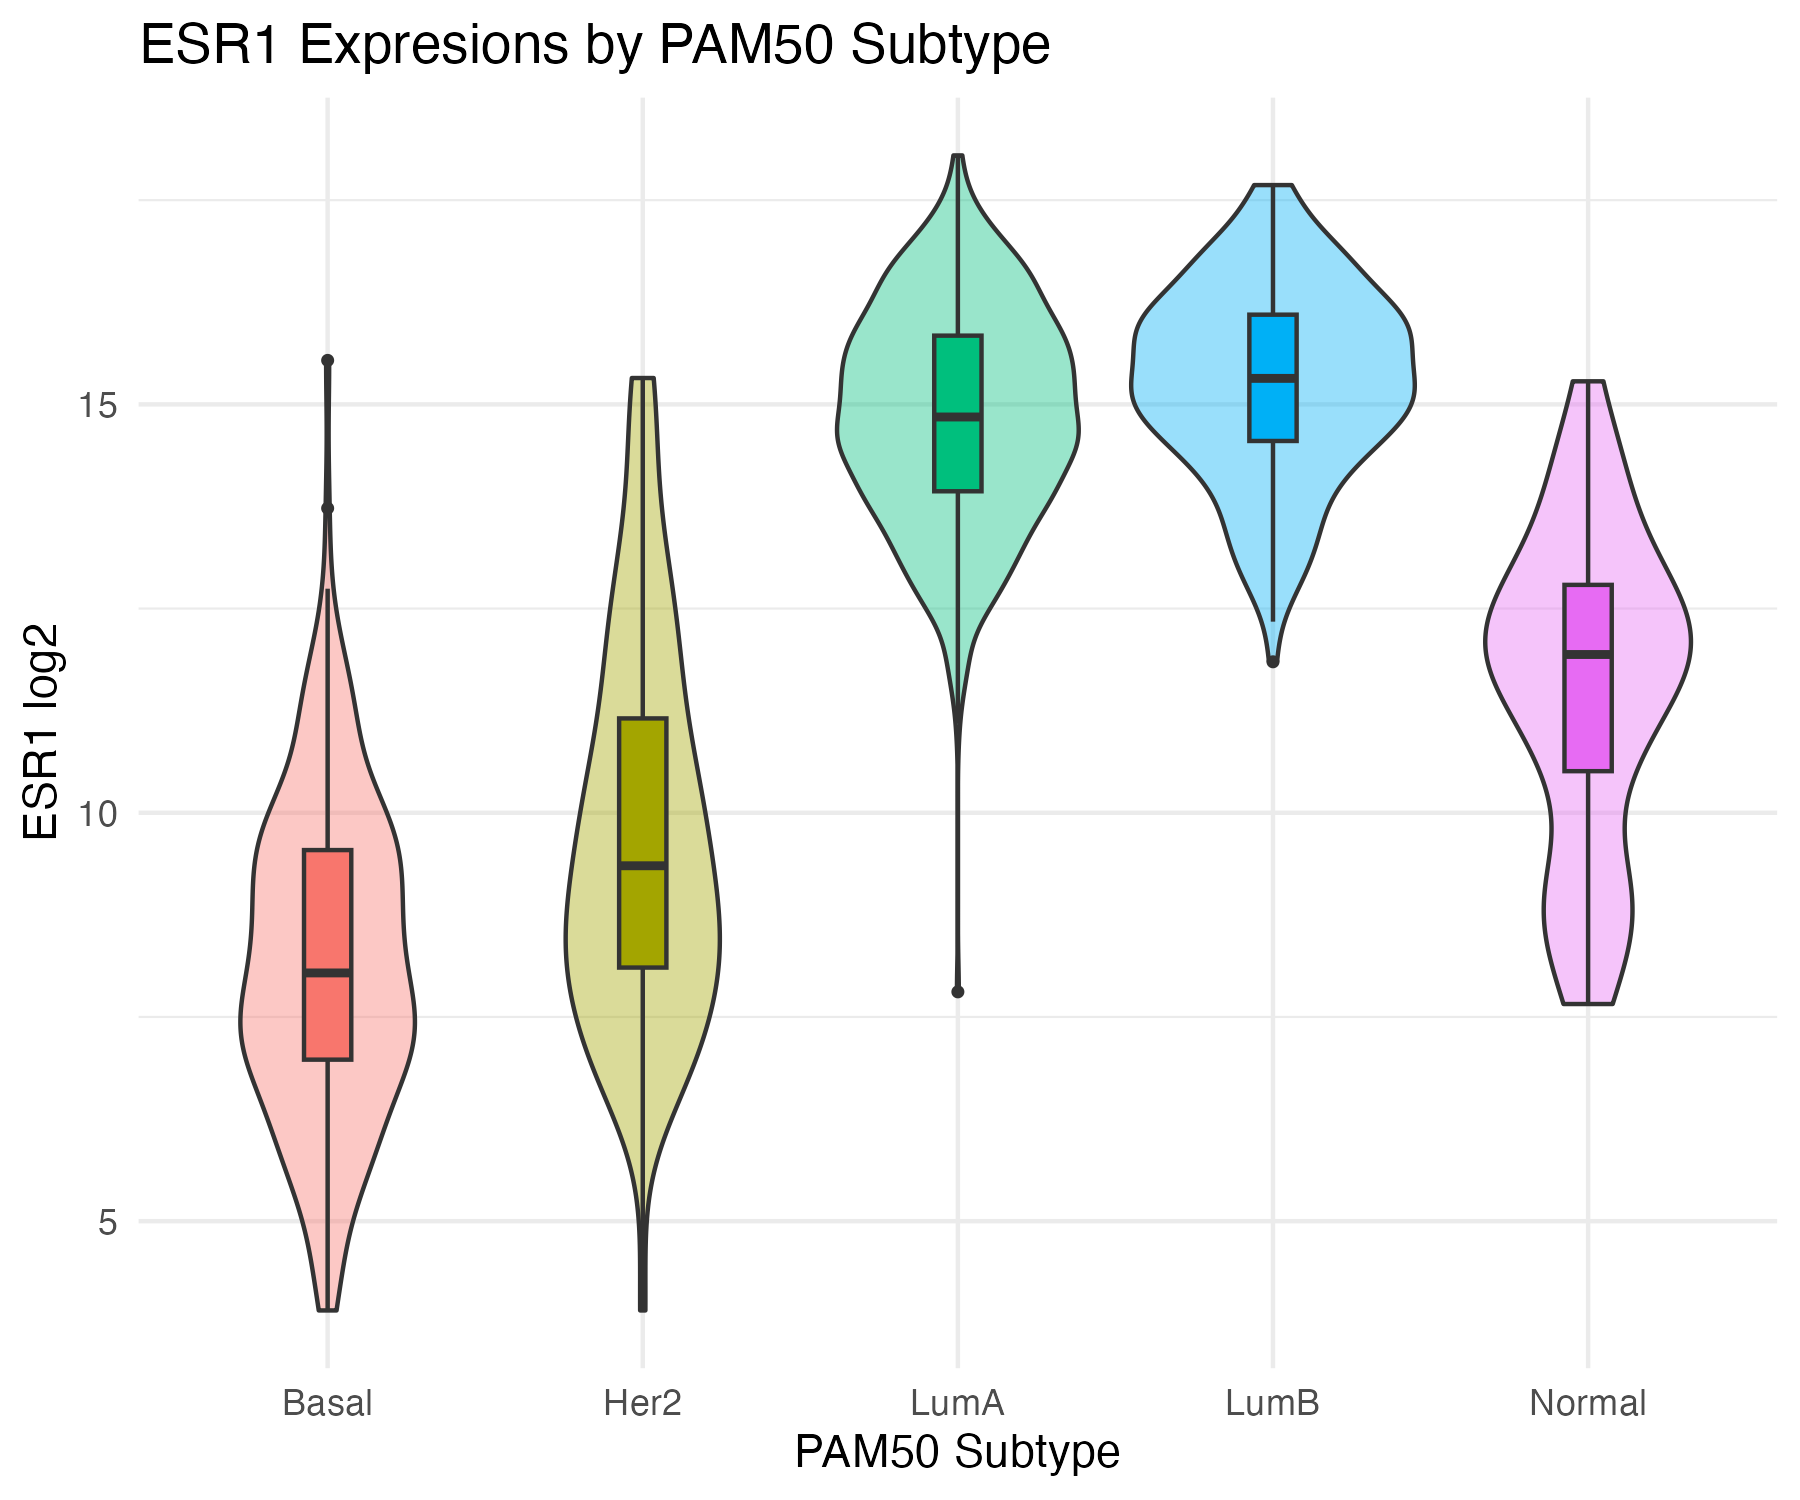
\includegraphics[width=0.75\textwidth]{figures/box_plot.png}
\caption{\textit{ESR1} expression by PAM50 subtype.}
\label{fig:box}
\end{figure}
\textit{ESR1} expression differed strongly by PAM50 subtype. LumA and LumB  had the highest expression, followed by the Normal-like group, while Her2 and Basal had the lowest. This explains known biology: luminal tumors are estrogen receptor-positive, while basal tumors are typically estrogen receptor negative.
\subsection{Heatmap}
\begin{figure}[H]
\centering
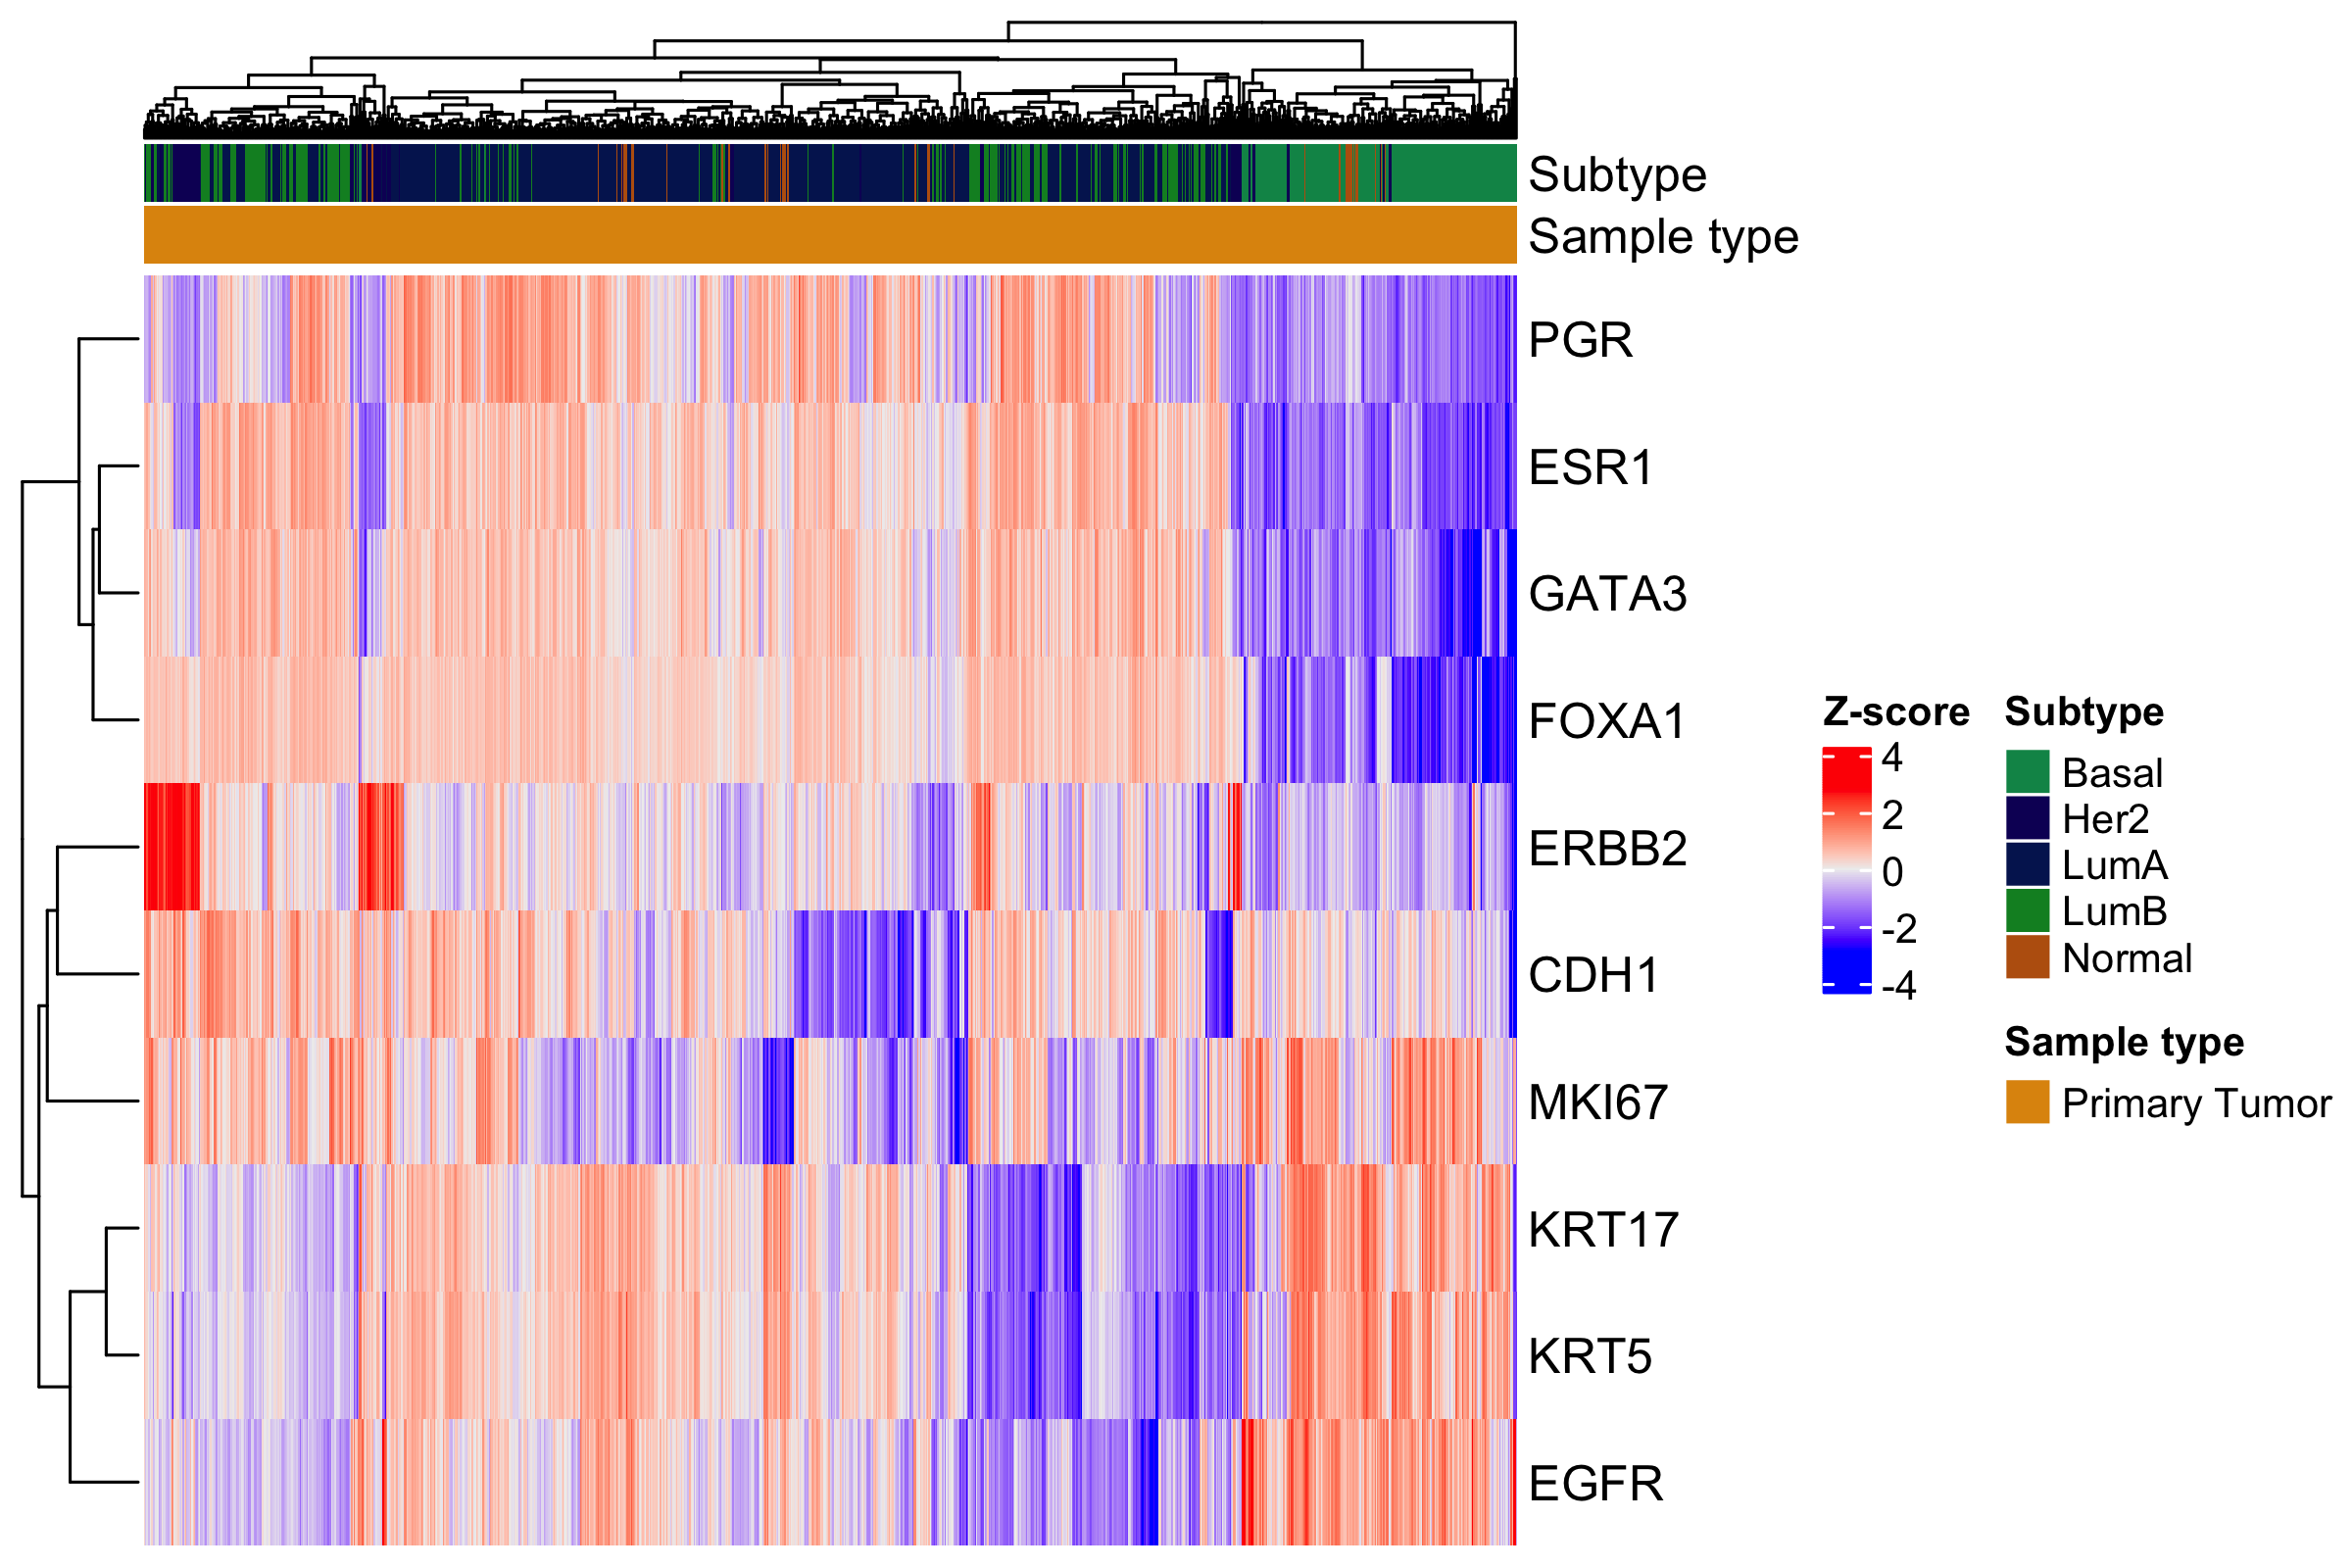
\includegraphics[width=\textwidth]{figures/heatmap.png}
\caption{Heatmap of row-scaled expression for 10 genes}
\label{fig:heat}
\end{figure}
One group of samples showed high expression of luminal markers (\textit{ESR1}, \textit{GATA3}, \textit{FOXA1}, \textit{PGR}), while the other showed low expression of these genes together with high expression of the basal markers \textit{KRT5}, \textit{KRT17}, and \textit{EGFR}. \textit{ERBB2} was  elevated in a small set of samples, consistent with the HER2 enriched subtype. All samples were primary tumors, so the sample type shows a single category.

\subsection{\textit{ESR1} density by PAM50 subtype}
\begin{figure}[H]
\centering
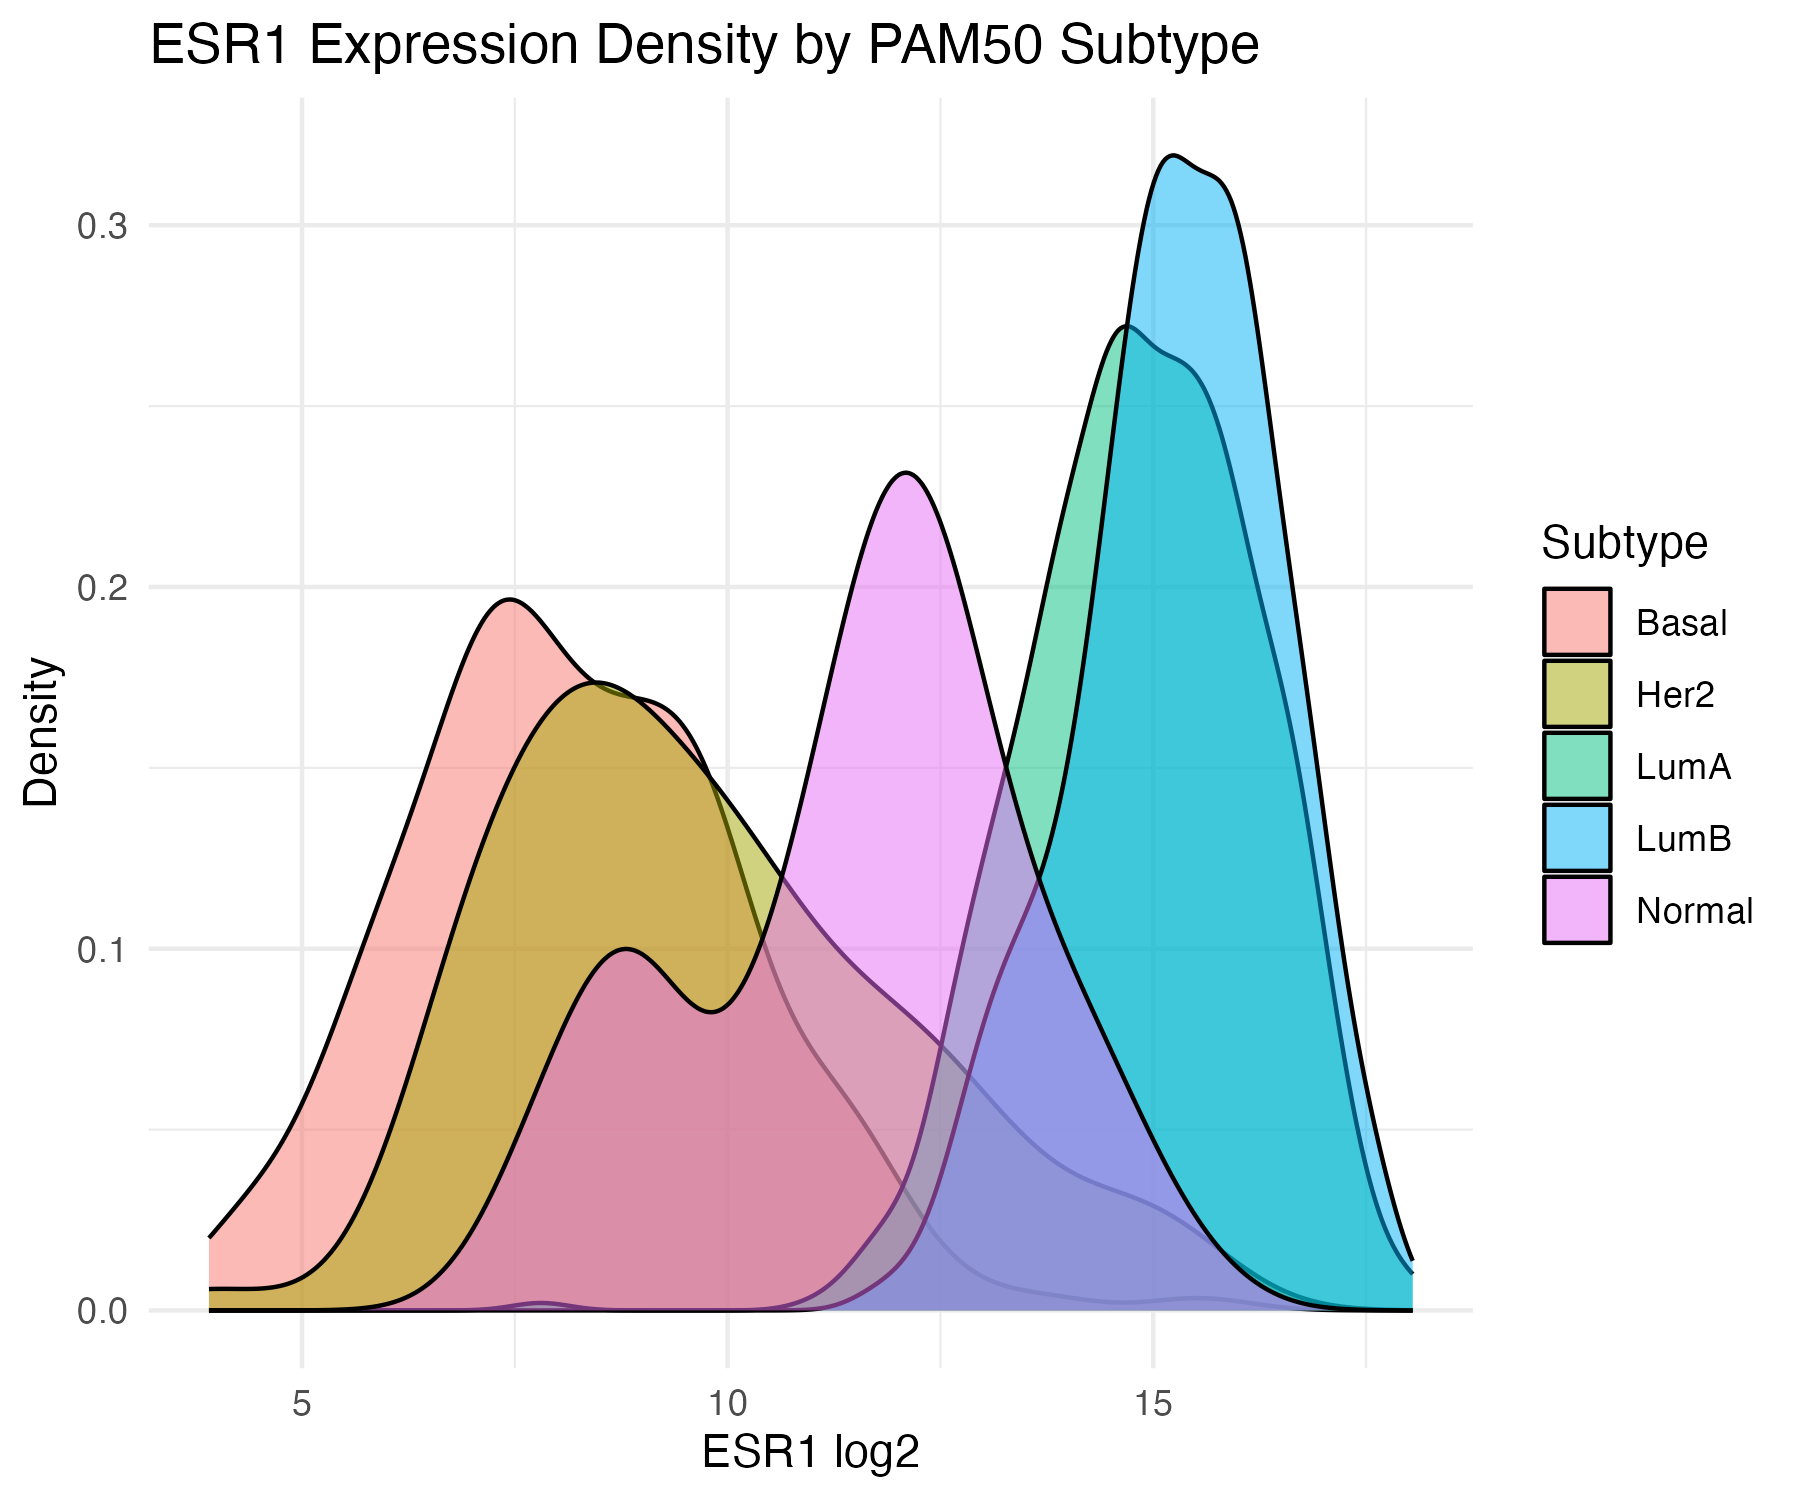
\includegraphics[width=0.8\textwidth]{figures/density_plot.png}
\caption{Density of \textit{ESR1} expression by PAM50 subtype.}
\label{fig:density}
\end{figure}
The density plot shows the same separation as the box plot in more detail. Basal and Her2 overlap heavily at low expression, LumA and LumB overlap at high expression, and the Normal group sits in between with a single peak.

%---------------------------------------------------------------
\newpage
\begin{thebibliography}{9}

\bibitem{tcga2012}
The Cancer Genome Atlas Network. Comprehensive molecular portraits of human breast tumours. \textit{Nature}. 2012;490:61--70.

\bibitem{grossman2016}
Grossman RL, et al. Toward a shared vision for cancer genomic data. \textit{New England Journal of Medicine}. 2016;375:1109--1112. Data from the NCI Genomic Data Commons, project TCGA-BRCA. \url{https://portal.gdc.cancer.gov}

\bibitem{parker2009}
Parker JS, et al. Supervised risk predictor of breast cancer based on intrinsic subtypes. \textit{Journal of Clinical Oncology}. 2009;27(8):1160--1167.

\bibitem{wickham2016}
Wickham H. \textit{ggplot2: Elegant Graphics for Data Analysis}. Springer-Verlag New York; 2016.

\bibitem{gu2016}
Gu Z, Eils R, Schlesner M. Complex heatmaps reveal patterns and correlations in multidimensional genomic data. \textit{Bioinformatics}. 2016;32(18):2847--2849.

\bibitem{guBook}
Gu Z. \textit{ComplexHeatmap Complete Reference}. \url{https://jokergoo.github.io/ComplexHeatmap-reference/book/}. Accessed October 2026.

\bibitem{courseData}
Course-provided RNA-seq count matrix (counts.csv) and sample metadata (meta\_data.csv), TCGA-BRCA cohort. Data from The Cancer Genome Atlas (TCGA), a program of the National Cancer Institute (NCI) and the National Human Genome Research Institute (NHGRI).

\end{thebibliography}

\end{document}